\section{Statements and Functions} \label{sect:statements-and-functions}

\subsection*{Comparison}

JS의 equality comparison은 여타 언어들과 유사하게 \texttt{==}과 \texttt{!=} 연산자로 수행될 수 있으며, 비교 연산의 결과가 참이면 \texttt{true}, 거짓이면 \texttt{false}를 반환한다. 그러나 JS에서는 \texttt{==}이나 \texttt{!=} 연산자로 비교 연산을 수행하였을 때 문제가 발생할 수 있다.

\begin{codeenv}{code:loose-equality}{Loose Equality}\begin{verbatim}


> 0 == 0;
true
> 0 == '0';
true
\end{verbatim}
\end{codeenv}

\coderef{code:loose-equality}에서는 number형의 \texttt{0}과 string형의 \texttt{'0'}을 비교하였다. 두 값은 자료형이 다름에도 불구하고 같다는 결과가 도출되는데, 그 이유는 JS에서 \texttt{==}과 \texttt{!=} 연산자를 이용하여 비교 연산을 수행할 때, 두 값에 대해 자의적으로 자료형 변환(type coercion)을 수행한 뒤 변환된 값을 비교하기 때문이다. 이렇게 비교 연산에서 \texttt{==}과 \texttt{!=} 연산자를 사용하여 자료형 변환이 이루어진 뒤 수행되는 연산을 loose equality이라고 한다. JS가 수행하는 타입 변환 규칙은 복잡하기 때문에 loose equality는 사용하지 않는 것이 권장된다.

\begin{figure}[htb]\vspace{10pt}\centering
    \begin{subfigure}{.231\textwidth}\centering
        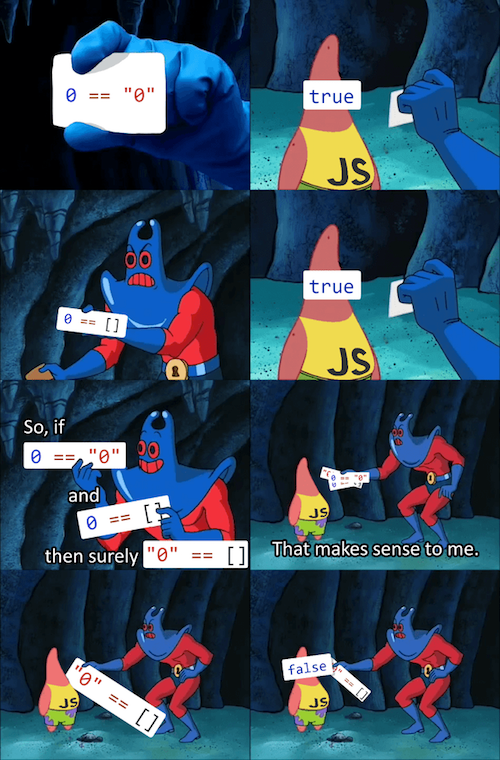
\includegraphics[width=\textwidth]{images/basics-of-javascript/loose-equality-syllogism.png}
        \caption{Syllogism does not hold}
        \label{fig:loose-equality-syllogism}
    \end{subfigure}
    \begin{subfigure}{.729\textwidth}\centering
        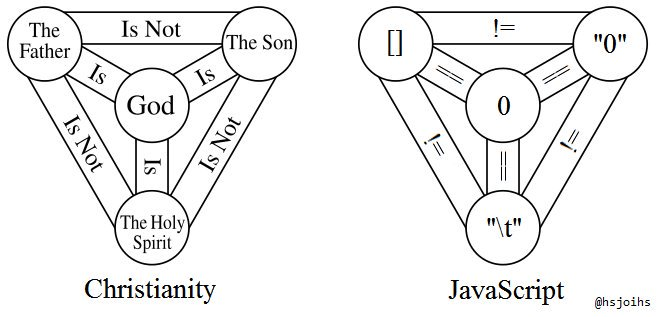
\includegraphics[width=\textwidth]{images/basics-of-javascript/loose-equality-trinity.jpg}
        \caption{The Javascript Trinity of \texttt{0}}
        \label{fig:loose-equality-trinity}
    \end{subfigure}
    \caption{Loose Equality Memes}
    \label{fig:loose-equality-memes}
\end{figure}

이러한 이유로 JS에서는 loose equality 대신 자료형까지 고려하여 값을 비교하는 strict equality가 권장된다. Strict equality는 \texttt{===}과 \texttt{!==} 연산자를 이용하여 수행될 수 있다.

\begin{codeenv}{code:strict-equality}{Strict Equality}\begin{verbatim}


> 0 === 0;
true
> 0 === '0';
false
\end{verbatim}
\end{codeenv}

\figref{fig:comparison-table}는 loose equality와 strict equality의 결과를 정리한 표이다. 이 결과를 알아두어서 나쁠 것은 없지만, 가독성이 좋고 논리적 오류를 최소화할 수 있는 strict equality를 사용하는 것이 훨씬 효율적이다.

\begin{figure}[htb]\vspace{10pt}\centering
    \begin{subfigure}{.48\textwidth}\centering
        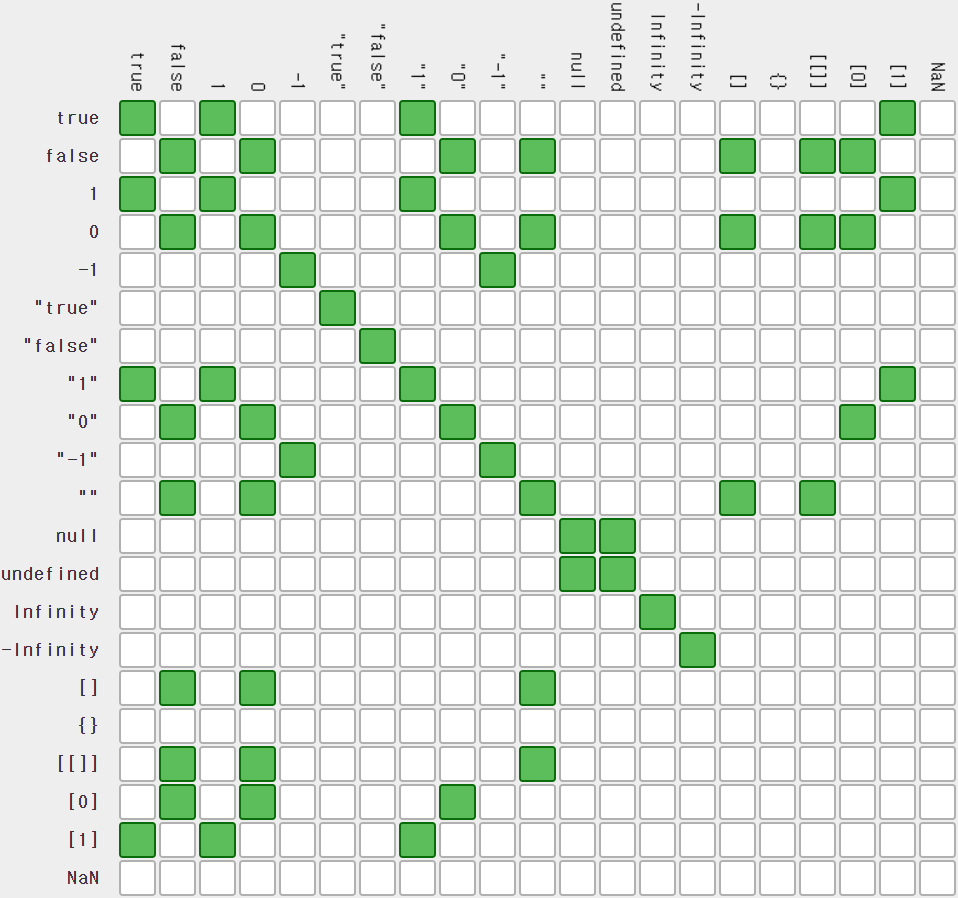
\includegraphics[width=\textwidth]{images/basics-of-javascript/loose-equality.png}
        \caption{Loose Equality}
        \label{fig:loose-equality-table}
    \end{subfigure}
    \begin{subfigure}{.48\textwidth}\centering
        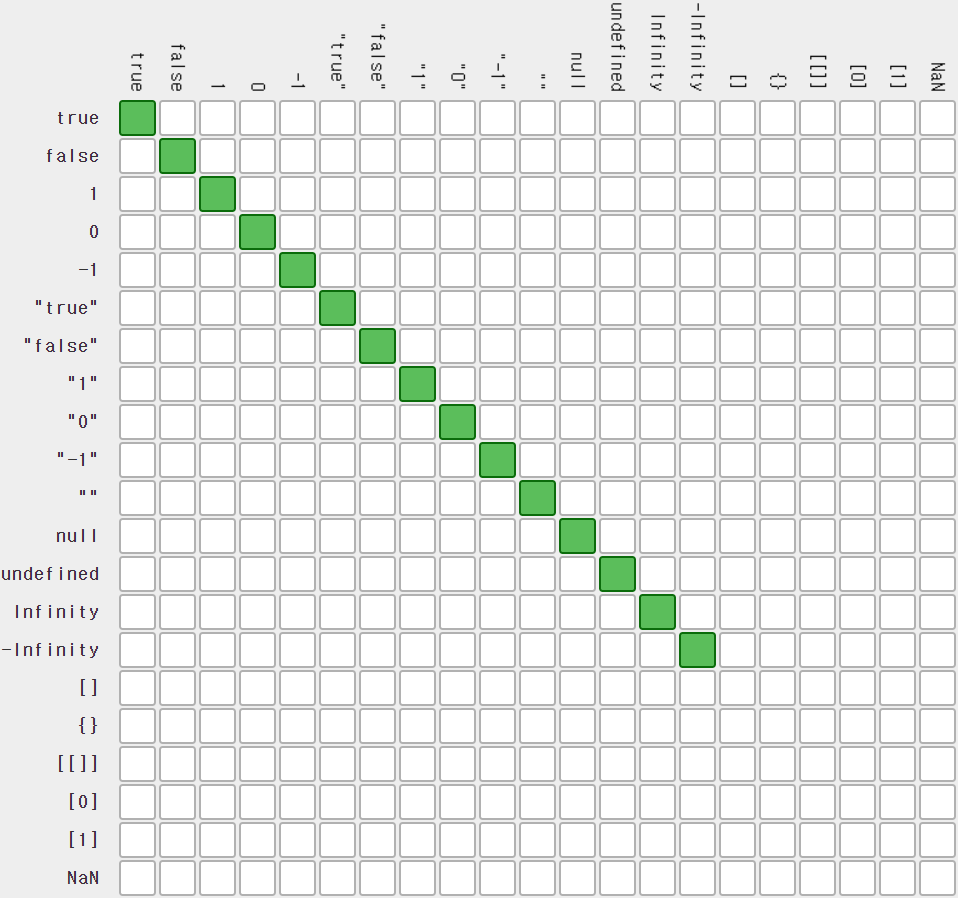
\includegraphics[width=\textwidth]{images/basics-of-javascript/strict-equality.png}
        \caption{Strict Equality}
        \label{fig:strict-equality-table}
    \end{subfigure}
    \caption{Equality table of JS. Colored cell implies \texttt{true}\protect\footnotemark}
    \label{fig:comparison-table}
\end{figure}

\footnotetext{https://dorey.github.io/JavaScript-Equality-Table/}

MDN 문서\footnote{https://developer.mozilla.org/en-US/docs/Web/JavaScript/Equality\_comparisons\_and\_sameness}를 참고하면 equality comparison에 대해 더 자세한 내용을 확인할 수 있다.

\subsection*{Conditional Statements}

JS의 조건문은 여타 언어들의 조건문과 유사하게 \texttt{if}, \texttt{if else}, \texttt{else}의 키워드를 사용한다.

\begin{codeenv}{code:if-else-stmt}{If-else Statement}\begin{verbatim}


> const num = 100;
> const isEven = num % 2 === 0;
> if (isEven) {
      console.log('num is even');
  } else {
      console.log('num is odd');
  }
num is even
> const remainder = num % 3;
> if (remainder === 0) {
      console.log('remainder is 0');
  } else if (remainder === 1) {
      console.log('remainder is 1');
  } else {
      console.log('remainder is 2');
  }
remainder is 1
\end{verbatim}
\end{codeenv}
\newpage

또한, switch-case문과 삼항 연산자 \texttt{? :}도 지원한다.

\begin{codeenv}{code:switch-case-stmt-ternary}{switch-case Statement and Ternary operator}\begin{verbatim}


> const num = 100;
> const remainder = num % 3;
> switch (remainder) {
      case 1:
          console.log('remainder is 1'); break;
      case 2:
          console.log('remainder is 2'); break;
      default:
          console.log('remainder is 0');
  }
remainder is 1
> const quotient = ((num % 7 === 0) ? num : (num - num % 7)) / 7;
14
\end{verbatim}
\end{codeenv}

\subsection*{Iteration Statements}

JS의 반복문 역시 여타 언어들과 유사하게 for문을 사용하며, while문과 do-while문 역시 지원한다.

\begin{codeenv}{code:for-stmt}{for Statement}\begin{verbatim}


> const fruits = ['apple', 'orange', 'mango', 'grapes'];
> for (let i = 0; i < fruits.length; i++) {
      console.log(fruits[i]);
  }
apple
orange
mango
grapes
\end{verbatim}
\end{codeenv}

\coderef{code:for-stmt}와 같이 반복문을 사용할 때마다 배열의 index를 어떠한 변수에 저장하고, 이를 이용해 배열의 각 원소를 가져오는 것은 번거롭다. for-of문을 사용하여 반복문을 간결하게 사용할 수 있다.

\begin{codeenv}{code:for-of-stmt}{for-of Statement}\begin{verbatim}


> const fruits = ['apple', 'orange', 'mango', 'grapes'];
> for (const fruit of fruits) {
    console.log(fruit);
}
apple
orange
mango
grapes
\end{verbatim}
\end{codeenv}

\coderef{code:for-of-stmt}과 같이 for-of문은 배열의 각 원소를 차례대로 특정 변수(\texttt{fruit})에 저장하고, for문 내에서 사용할 수 있도록 한다. 이렇게 for-of문을 사용하면 각 원소의 index는 알 수 없지만, 개별 원소는 직접 가져와 반복문을 간결하게 작성할 수 있는 장점이 있다.

\begin{codeenv}{code:for-in-stmt}{for-in Statement}\begin{verbatim}


> const person = { age: 21, name: 'Frank', height: 171, isMale: true, weight: 60 };
> for (const key in person) {
      console.log(key + ': ' + person[key]);
  }
age: 21
name: Frank
height: 171
isMale: true
weight: 60
\end{verbatim}
\end{codeenv}

for-of문과 유사하여 헷갈리기 쉬운 for-in문은 객체(object)에 대해 동작하며, for-in문 내부에서 객체의 각 key를 직접 가져와 사용할 수 있고, 이를 이용해 value에도 바로 접근할 수 있다.

\subsection*{Functions}

\begin{codeenv}{code:basic-function}{Function Declaration and Call}\begin{verbatim}


> function add(x, y) {
      return x + y;
  }
> add(1, 2);
3
> add('1', '2');
'12'
\end{verbatim}
\end{codeenv}

JS에서 함수는 \coderef{code:basic-function}와 같이 \texttt{function} 키워드를 이용하여 함수의 이름과 인자를 작성하고, 중괄호 내부에 함수 내용을 작성한다. JS에서는 식별자의 자료형을 따로 지정하지 않으므로 인자와 반환값의 자료형 역시 따로 지정하지 않는다는 점을 주목하여야 한다. 따라서, \coderef{code:basic-function}의 함수는 마지막 줄과 같이 사용될 수도 있다.

\begin{codeenv}{code:arrow-function}{Arrow Function}\begin{verbatim}


> const add = (x, y) => {
      return x + y;
  };
> add(1, 2);
3
> const square = num => num * num;
> square(5);
25
\end{verbatim}
\end{codeenv}

ES6 이후에는 \coderef{code:arrow-function}과 같이 arrow(\texttt{=>})를 사용하여 함수를 비교적 간결하게 정의하는 것이 권장된다. 표현식을 관찰해보면, \texttt{x}와 \texttt{y} 두 인자를 받아 덧셈을 수행한 뒤 반환하는 함수를 \texttt{add}라는 식별자에 할당하였다. JS에서는 함수 역시 하나의 변수 또는 상수로 취급될 수 있어 arrow function을 이용하여 함수를 작성할 수 있고, 함수를 다른 함수의 인자로 넘길 수도 있다.

Arrow function의 인자가 1개일 때는 인자 부분의 괄호를 생략할 수 있고, 함수에 값을 반환하는 부분만 있는 경우 중괄호와 \texttt{return} 키워드가 생략될 수 있다.

\begin{codeenv}{code:anonymous-function}{Anonymous Function}\begin{verbatim}


> num => num * num;
function (num)
> ((base, power) => {
      res = 1;
      for (let i = 0; i < power; i++) res *= base;
      return res;
  })(3, 5);
243
\end{verbatim}
\end{codeenv}

Arrow function을 활용하면 \coderef{code:anonymous-function}와 같이 익명 함수(anonymous function)를 선언할 수 있다.

\begin{codeenv}{code:high-order-function}{Anonymous Function with High-order Function}\begin{verbatim}


> const arr = ['a', 'bb', 'ccc', 'dddd'];
> const lengths = arr.map(e => e.length);
> lengths;
[ 1, 2, 3, 4 ]
\end{verbatim}
\end{codeenv}

함수 중에는 함수를 인자로 쓰는 함수가 있는데, 이러한 함수를 고차원 함수(high-order function)라고 한다. 익명 함수는 재사용하지 않는 함수를 고차원 함수의 인자로 넘길 때 유용하게 사용된다. \coderef{code:high-order-function}에서 \texttt{map} 함수는 배열의 각 원소를 인자로 받은 함수의 인자로 주어 실행한 결과를 배열로 반환한다. JS에서는 이러한 고차원 함수가 특히 많으므로 고차원 함수를 사용하면서 익명 함수를 빈번하게 사용하게 될 것이다.

\begin{codeenv}{code:foreach-method}{\texttt{forEach} Method}\begin{verbatim}


> const fruits = ['apple', 'orange', 'mango', 'grapes'];
> fruits.forEach(fruit => console.log(fruit));
apple
orange
mango
grapes
> const printFruit = (fruit, idx) => console.log('#' + (idx + 1) + ': ' + fruit);
> fruits.forEach(printFruit);
#1: apple
#2: orange
#3: mango
#4: grapes
\end{verbatim}
\end{codeenv}

익명 함수를 이용하여, 앞에서 다룬 for-of 문을 \coderef{code:foreach-method}과 같이 \texttt{forEach} 함수를 사용하여 바꿀 수 있다. \texttt{forEach} 함수는 각 원소뿐만 아니라 원소의 index와 원본 배열까지도 받아 사용할 수 있다.
